\section{Diodes}\label{sec:Diodes}
A \nameref{def:Diode} is one of the basic building blocks for almost all analog circuit systems.

\begin{definition}[Diode]\label{def:Diode}
  A \emph{diode} is a 2-port non-linear circuit element.
  Its circuit symbol is shown in \Cref{fig:Diode_Circuit_Symbol}.
\end{definition}

\begin{figure}[h!tbp]
  \centering
  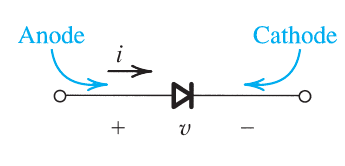
\includegraphics[scale=0.75]{./Diode_Circuit_Symbol.png}
  \caption{Diode Circuit Symbol \parencite[p.~177]{sedraTextbook7}}
  \label{fig:Diode_Circuit_Symbol}
\end{figure}

An \textbf{ideal diode} is one that behaves as a short-circuit when a voltage applied is forward-biased, and acts as an open-circuit with the voltage is reverse-biased.
The current-voltage characteristic is shown in \Cref{fig:Ideal_Diode_IV_Characteristic}.

\begin{figure}[h!tbp]
  \centering
  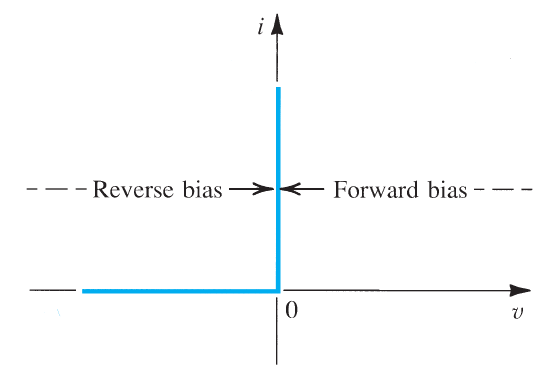
\includegraphics[scale=0.75]{./Ideal_Diode_IV_Characteristic.png}
  \caption{Ideal Diode \DCCurrent{}-\DCVoltage{} Characteristic \parencite[p.~177]{sedraTextbook7}}
  \label{fig:Ideal_Diode_IV_Characteristic}
\end{figure}

\subsection{Terminal Characteristics of Junction Diodes}\label{subsec:Terminal_Characteristics_Junction_Diodes}
A \textbf{junction diode} is a \nameref{def:Diode} built using a \PNJunction{}.
In this case, there are three distinct regions in the characteristic curve:
\begin{enumerate}[noitemsep]
\item \nameref{subsubsec:Diode_Forward-Bias_Region}, where $\Voltage > 0$.
\item \nameref{subsubsec:Diode_Reverse-Bias_Region}, where $\Voltage < 0$.
\item \nameref{subsubsec:Diode_Breakdown_Region}, where $\Voltage < - \ReverseBreakdownVoltage$.
\end{enumerate}

\subsubsection{The Forward-Bias Region}\label{subsubsec:Diode_Forward-Bias_Region}
The forward-bias region is the one where the terminal voltage $\Voltage$ is positive.

In the forward region, we can approximate the current-voltage relationship by using \Cref{eq:pn-Junction-Current-Voltage_Relation-Simple}, with minor modifications, as seen in \Cref{eq:Diode_Forward-Bias-IV_Relationship}.

\begin{equation}\label{eq:Diode_Forward-Bias-IV_Relationship}
  \Current = \SaturationCurrent \left( e^{\frac{\Voltage}{\ThermalVoltage}} - 1 \right)
\end{equation}

There is a slightly \textbf{more} modified version, in \Cref{eq:Diode_Forward-Bias-IV_Relationship-n}

\begin{equation}\label{eq:Diode_Forward-Bias-IV_Relationship-n}
  \Current = \SaturationCurrent \left( e^{\frac{\Voltage}{n \ThermalVoltage}} - 1 \right)
\end{equation}

$n$ has a value between 1 and 2.
$n$ is a number that depends on the material and physical structure of the diode.
From here-on-out, we assume that $n = 1$.
However, there may be cases when you should use a different $v$ value instead.

If the diode has $\Current \gg \SaturationCurrent$, then we can approximate \Cref{eq:Diode_Forward-Bias-IV_Relationship} using \Cref{eq:Diode_Forward-Bias-IV_Relationship-Approximate}.

\begin{equation}\label{eq:Diode_Forward-Bias-IV_Relationship-Approximate}
  \Current \simeq \SaturationCurrent e^{\frac{\Voltage}{\ThermalVoltage}}
\end{equation}

The relationship in \Cref{eq:Diode_Forward-Bias-IV_Relationship-Approximate} can be expressed in terms of currents instead of voltages as well.
\begin{equation}\label{eq:Diode_Forward-Bias-VI_Relationship-Approximate}
  \Voltage = \ThermalVoltage \ln \left( \frac{\Current}{\SaturationCurrent} \right)
\end{equation}

\subsubsection{The Reverse-Bias Region}\label{subsubsec:Diode_Reverse-Bias_Region}
In the reverse-bias region, the voltage applied to the \nameref{def:Diode} is in the reverse direction.
This causes the diode to behave \emph{like} an open-circuit.
However, this is not technically true, because a small amount of current does ``leak'' out, as seen by \Cref{eq:Diode_Reverse-Bias-Current_Relation}.

\begin{equation}\label{eq:Diode_Reverse-Bias-Current_Relation}
  \Current \simeq - \SaturationCurrent
\end{equation}

\subsubsection{The Breakdown Region}\label{subsubsec:Diode_Breakdown_Region}
Lastly, the breakdown region is where the voltage applied in the reverse-bias direction is so great, that the \nameref{def:Diode} starts working in reverse, conducting current in the reverse direction.
This region will be discussed much more in the section devoted to \nameref{subsec:Zener_Diodes}.

\subsection{Modeling the Diode's Forward Characteristic}\label{subsec:Modeling_Diode_Forward_Characteristic}
There are several different models, appropriate at different times of analysis.

\subsubsection{The Exponential Model}\label{subsubsec:Exponential_Diode_Model}
In the exponential model of a \nameref{def:Diode}, you use the diode's current-voltage characteristic and another equation containing the current through the diode and the voltage across the diode to solve for $\DCCurrent{D}$ and $\DCVoltage{D}$.

The downside to this model is that it can require a lot of knowledge about the \nameref{def:Diode} and its properties.
In addition, because an exponential function $\DCCurrent{D} = \SaturationCurrent e^{\frac{\DCVoltage{D}}{\ThermalVoltage}}$ and a linear function are being used to find a solution, finding that solution can be computationally difficult.
Due to this, it is only used in the final stages of circuit development/analysis and is not much discussed in either this document or this course.
Instead, we focus on ways to more quickly model a \nameref{def:Diode} and its characteristics.

\subsubsection{The Constant-Voltage-Drop Model}\label{subsubsec:Constant_Voltage_Drop_Diode_Model}
In the constant-voltage-drop model, we assume the \nameref{def:Diode} is semi-ideal.
Meaning that we approximate the real exponential function, $\DCCurrent{D} = \SaturationCurrent e^{\frac{\DCVoltage{D}}{\ThermalVoltage}}$ to a piecewise linear one.
The constant-voltage-drop model for a silicon-based diode is shown in \Cref{fig:Silicon_Diode_Constant_Voltage_Drop}.

\begin{figure}[h!tbp]
  \centering
  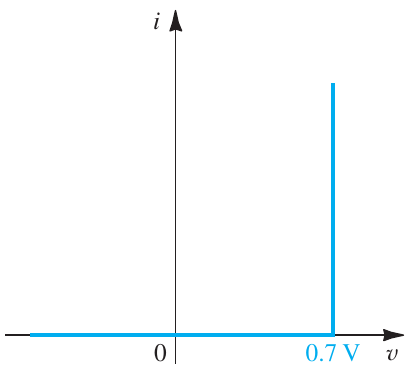
\includegraphics[scale=0.75]{./Silicon_Diode_Constant_Voltage_Drop}
  \caption{Silicon Diode Constant-Voltage-Drop Model \parencite[p.~193]{sedraTextbook7}}
  \label{fig:Silicon_Diode_Constant_Voltage_Drop}
\end{figure}

Essentially, this simplifies a \nameref{def:Diode} down to a DC voltage source, where the source's positive terminal is on the anode of the diode.
This source can then be used when performing circuit analysis to get reasonably accurate answers for the amount of work required.

\subsubsection{The Ideal Diode Model}\label{subsubsec:Ideal_Diode_Model}
In the ideal diode model, it is assumed that the \nameref{def:Diode} in question \textbf{is} ideal.
This means that if the voltage across the diode is greater than zero, the diode acts as a short-circuit.
This can be seen graphically in \Cref{fig:Ideal_Diode_IV_Characteristic}.

\subsubsection{The Small-Signal Model}\label{subsubsec:Diode_Small-Signal_Model}
In the small-signal model, we are interested in how small changes across the \nameref{def:Diode} affect its properties.
For example, say we increase the original source voltage $\Voltage_{S}$ by $\Delta \Voltage_{DD}$, we would be interested in the change in the diode's current and voltage.

To solve this, we actually use the exponential model, but we are only concerned with the highest one or two orders in the infinite summation.

\begin{blackbox}
  Remember that Euler's exponential can be represented using an infinite series, seen below:
  \begin{align*}
    e^{x} &= 1 + x + \frac{x^{2}}{2!} + \frac{x^{3}}{3!} + \cdots \\
    &= \sum\limits_{k = 0}^{\infty} \frac{x^{k}}{k!}
  \end{align*}
\end{blackbox}

If we are working with a small enough change ($\Delta \Voltage_{DD} \ll \ThermalVoltage$), then the exponential curve is dominated by the $1+x$ term in the infinite series.

To simplify the explanations here, we will pretend that the $\Delta \Voltage_{DD}$ is actually an AC voltage, $\ACVoltage{d}(t)$.

\begin{align*}
  \intertext{Then, by the theory of superposition, the voltage across the diode is also a time-varying function shown below.}
  \ACVoltage{D}(t) &= \DCVoltage{D} + \ACVoltage{d}(t) \\
  \intertext{Knowing how a \nameref{def:Diode} works, we can say,}
  \ACCurrent{D}(t) &= \SaturationCurrent e^{\frac{\ACVoltage{D}}{\ThermalVoltage}} \\
  \shortintertext{Substitute for $\ACVoltage{D}(t)$} \\
                   &= \SaturationCurrent e^{\frac{\DCVoltage{D} + \ACVoltage{d}(t)}{\ThermalVoltage}} \\
                   &= \SaturationCurrent e^{\frac{\DCVoltage{D}}{\ThermalVoltage}} e^{\frac{\ACVoltage{d}(t)}{\ThermalVoltage}} \\
  \intertext{Let $\DCCurrent{D} = \SaturationCurrent e^{\frac{\DCVoltage{D}}{\ThermalVoltage}}$.}
  \ACCurrent{D}(t) &= \DCCurrent{D} e^{\frac{\ACVoltage{d}(t)}{\ThermalVoltage}} \\
  \intertext{If we keep the amplitude of the change we introduce remain small, meaning the $e^{\frac{\ACVoltage{d}(t)}{\ThermalVoltage}} \approx 1$, then we can solve this.
  Such a constraint means that $\frac{\ACVoltage{d}(t)}{\ThermalVoltage} \ll 1$.
  Expanding the exponential using its infinite series and truncating after two terms yields a reasonable approximation.
  In that case:}
  \ACCurrent{D}(t) &\simeq \DCCurrent{D} \left( 1 + \frac{\ACVoltage{d}(t)}{\ThermalVoltage} \right) \\
\end{align*}

This last derivation is important, because it is the \textbf{small-signal approximation}.
I have restated it here to demonstrate just \emph{how} important it is.

\begin{equation}\label{eq:Diode_Small-Signal_Approximation}
  \ACCurrent{D}(t) \simeq \DCCurrent{D} \left( 1 + \frac{\ACVoltage{d}(t)}{\ThermalVoltage} \right)
\end{equation}


%%% Local Variables:
%%% mode: latex
%%% TeX-master: "../ECE_311-Engineering_Electronics-Reference_Sheet"
%%% End:
